\documentclass[11pt,a4paper]{article}
\usepackage{titlesec} %these are how we import packages, one helps set up footers and title layout
\usepackage{fancyhdr}
\usepackage{titlesec}
\usepackage{lipsum}
\usepackage[final]{pdfpages}
\usepackage[textsize=tiny]{todonotes}
\usepackage{apacite}
\usepackage[hyphens,spaces,obeyspaces]{url}
\usepackage{subfig}
\usepackage[utf8]{inputenc} % set input encoding (not needed with XeLaTeX)
\usepackage{graphicx} % support the \includegraphics command and options
\graphicspath{{./images/}}
\usepackage{csvsimple}
\usepackage[textsize=tiny]{todonotes}
\usepackage{textcomp}
\graphicspath{{./images/}}

\usepackage{booktabs} % for much better looking tables
\usepackage{array} % for better arrays (eg matrices) in maths
\usepackage{paralist} % very flexible & customisable lists (eg. enumerate/itemize, etc.)
\usepackage{verbatim} % adds environment for commenting out blocks of text & for better verbatim
\usepackage{subfig} % make it possible to include more than one captioned figure/table in a single float
\usepackage[toc,page]{appendix}
\usepackage{fontspec}
\usepackage[margin=1.0in]{geometry}
\setmainfont{Arial}

\pagestyle{fancyplain}
\fancyhf{}
\renewcommand{\headrulewidth}{0.5pt}
\renewcommand{\footrulewidth}{0.5pt}
\setlength{\headheight}{15pt}
\fancyhead[L]{Connor Timmins}
\fancyhead[R]{40451571}
\fancyfoot[L]{}
\fancyfoot[C]{\thepage}

\begin{document}

\newcommand{\HRule}{\rule{\linewidth}{0.5mm}}

{\Large Emergent Computing for Optimisation Coursework\par}

\section{Approach}
In this report, we use an evolutionary algorithm to determine the optimal team in fantasy football league. This algorithm takes a set of potential solutions, evaluates their fitness, holds tournaments to select the best candidates, performs a crossover operation to produce offspring solutions that replace the existing population, occassionally mutates the offspring and repeats for a set number of iterations to determine our optimal solution of a team with a value of 2097. To facilitate this, we make use of the eaSimple algorithm provided by the DEAP library.

Solving an NP-hard combinatorial optimisation problem is very difficult to do in a reasonable time frame using traditional techniques as the input scales up. A number of approaches can be taken to find an optimal solution such as stochastic search algorithms like tabu search or evolutionary algorithms. We have chosen to use an evolutionary algorithm as our approach. Typical local-search or meta-heuristic algorithms such as tabu search are black-box algorithms but our problem contains enough information that we can attain more reliably optimal solutions using domain-specific information in an evolutionary approach. For example, as shown later, we can seed our solutions with known optimal team members. It also allows us to consider solutions outside the feasible search space that may provide a path to an optimal solution through the use of a penalty in our fitness evaluation.

To represent a candidate solution, we use an indirect representation where a gene in the solution refers to the position of a player on a list. This is as each player on a team that makes up a solution is associated with multiple pieces of information, all of which are important when evaluating fitness.
Each player has a cost, a value and a role on the team (Goalkeeper, Defender, Midfielder or Striker). By using an indirect representation, we can access this information as needed.

Additionally, the team size is set at 11 players. Were we to use a binary representation for example where the individual was the size of the number of players and where 1 represents that a player is on the team and a 0 not on the team, we would need to take care during crossover and mutation to ensure that the new individual is still a valid size. The indirect representation allows to easily respect this important constraint throughout the lifecycle of the algorithm.


\section{Algorithm/Operator Design}
\subsection{Initialisation}
We created a custom initialisation operator for this implementation. When initialising an individual, we respect all constraints. Most importantly, we respect the team size constraint. As our crossover and mutation operators do not affect the size of an individual, our initial population must respect this constraint or this unfit characteristic may spread with no remedy possible.

A team is generated from a random set of players, each being added to the team once at a time. Each addition is checked to see whether the addition would break any constraints and if a constraint is broken, the team is discarded and the process begins freshly anew. This allows us to seed the population with valid solutions, encouraging a quicker evolution. There is a potential loss in diversity and there is a risk that the population converges to a local optimum through seeding but as each attempt at creating a team draws from a new random set of players every time, we feel this effect is mitigated.

By looking at the provided player data, we recognised one player in particular as a stand out. Player 'SALAH, M', position 378 in the provided CSV and position 376 in our implementation lists, has a point value of 378, 97 higher than the next highest while only costing 12.9. This outlier has such a high value at a reasonable cost that we can infer that any optimal solution is likely to contain it. Empirically, we found we reached our optimal solution more rapidly by seeding all solutions with this player in the initial lineup.

\subsection{Crossover}
For crossover operations, we have opted to use "Two-Point Crossover". It has been shown that in knapsack problems, two point crossover is one of the best crossover operators \cite{Hakimi2016}. Our implementation uses the two point crossover provided by the DEAP library.

\subsection{Mutation}
We created a custom mutation operator for this implementation. An individual subject to this mutation will have one random player replaced with another random player not currently in the team, while keeping all values in the list unique unless the individual prior to mutation does not have all unique values. This is to encourage solutions in the candidate pool which respect our uniqueness constraint.

\subsection{Selection}
For selection, we used a tournament selection operator provided by the DEAP library. Empirically, we found that is performed better than a roulette mechanism or a best solution operation. We hold a selection tournament of 3 individuals. We found that this brought us higher average highest fitness values and a quicker convergence to an optimal solution.
\subsection{Fitness}
To evaluate the fitness of a candidate, the total value of all players in the candidate is summed. 
If the candidate breaks any constraints, we calculate a penalty to be subtracted from the total value of the candidate.
We do not consider the constraint of 11 players in our fitness function. This is as all our initial candidates are set to have only 11 values and the mutation and crossover operators do not affect this size therefore breaking this restraint would be unexpected behaviour that we have not seen in any of our experiments.
We consider that a failure to respect the constraints of teamroles and non-uniqueness to be equivalent per occurence. That is to say that, all other values being equal, a solution that has three goalkeepers (one is expected) and one that has one midfielder (minimum three expected) are equally distant from the feasible region of the search space in that they both have two values breaking constraints. To determine the true distance from the feasible region of the search space, we first determine the maximum number of potential violations possible. This allows us to scale the effect of violating constraints while never causing our effect to become a number greater than 1 which could lead to the penalty effect being beneficial to the individual. The subsequent effect of the penalty is equal to:

\begin{equation}
Penalty = totalValue * \frac{constraintViolations}{maxPossibleConstraintViolations}
\end{equation}

In our implementation, there is a maximum number of 10 possible constraint violations, that is 10 possible players in the team can be invalid. We assume that at least one player is valid as our initialisation, crossover and mutation operators ensure that any value in an individual does refer to a real player and there are no restrictions on individual player availability.

When a candidate breaks the constraint of spending under or equal to £100, we calculate a penalty relative to the value of all players summed.

\begin{equation}
Penalty = totalValue * \frac{|cost-maxCost|}{min(maxCost, |totalCost-maxCost|}
\end{equation}



The following is the equation used for calculating a penalty as a combination of the previous effects.
\begin{equation}
Penalty = totalValue * \frac{dist+constraintViolations}{diff+maxConstraintViolation}
\end{equation}
%
where dist = |cost-maxCost| and diff = min(maxCost, |totalCost-maxCost|)

The resulting final fitness of an individual candidate is calculated with the following:

\begin{equation}
Fitness= totalValue-Penalty
\end{equation}

\section{Experimental Design \& Analysis}
To measure the performance of our algorithm and find optimal hyperparameters, we conduct several experiments detailed below. Our problem requires a single best output and does not require repititious use. Therefore, we seek to find hyperparameters that maximise our fitness and not our success rate.

The adjustable inputs to the algorithm are as follows:
\begin{description}
\item[POPSIZE] Population Size
\item[MUTPB] Mutation Probability
\item[CXPB] Crossover Probability
\item[TOURNSIZE] Tournament Size
\end{description}

If not otherwise specified, the default parameters used are 200, 0.1, 0.8 and 4 respectively.
Note: all best fitness values are only considered if no constraints are broken.

\subsection{Population Size Effect on Fitness}
To test the effect of population size on fitness, we run the algorithm with a population size of 50 to 250 in a step of 50. At each population size, the algorithm is run 10 times and the best fitness in each run recorded. Results are shown in Fig  \ref{fig:popSizeFit}.

\begin{figure}
\centering
\subfloat[Mean Fitness]{{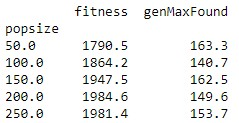
\includegraphics[width=0.3\textwidth]{PopFitness}}}
\qquad
\subfloat[Median Fitness]{{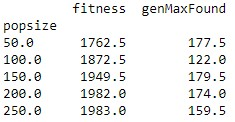
\includegraphics[width=0.3\textwidth]{PopMedian}}}
\caption{Population Size Data}
\label{fig:popSizeFit}
\end{figure}
Across all runs, we find a highest fitness value of 2042 occuring with a population size of 250. We see a highest mean fitness with population size 200 and second highest at 250. Applying a Shapiro-Wilk test, we get a result of 0.08 indicating that the population size 200 dataset does not have a normal distribution of fitness values. Applying the same test to population size 250, we get 0.7 indicating a normal distribution. We compare our median value for population size 200 (1982) and mean value for population size(1981.4), finding very similar values. 

Using a Kolmogorov-Smirnow test on these two sets, we get a very low value of 0.000217 indicating that these samples come from different distributions. As both are different distributions but produce very similar averages, we conclude that with our problem's need for highest possible value, population size set to 250 is most likely to produce our single most optimal result.

In subsequent experiments, we have set the population size to 250.

\subsection{Mutation Rate Effect on Fitness}
We test the effect of mutation rate on fitness by running the algorithm with a mutation rate 0.05 to 0.2 in a step of 0.05. At each mutation rate, the algorithm is run 10 times and the best fitness in each run recorded. Results are shown in Fig \ref{fig:mutRateFit}.

\begin{figure}
\centering
\subfloat[Mean Fitness]{{\includegraphics[width=0.3\textwidth]{mutMean}}}
\qquad
\subfloat[Median Fitness]{{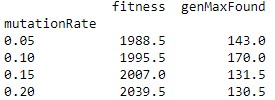
\includegraphics[width=0.3\textwidth]{mutMedian}}}
\caption{Mutation Rate Data}
\label{fig:mutRateFit}
\end{figure}

We find our highest fitness value of 2077 at a 0.2 mutation rate. Using a Shapiro-Wilk test, we get a result of 0.52 indicating a normal distribution but only slightly. As such, we choose to consider both mean and median values of 2028 and 2039. In both averages, there is a distance of over 20 fitness to the next nearest average fitness strongly showing the positive effect a higher mutation rate has on our problem.
This is expected as we choose to seed all solutions with a single best known player which is expected to reduce diversity and a high mutation rate reintroduces diversity. In subsequent experiments, the mutation rate is set to 0.2.

\subsection{Crossover Probability Effect on Fitness}
We test the effect of crossover probability on fitness by running the algorithm with a crossover probability of 0.8 to 1.0 in a step of 0.05. At each rate, the algorithm is run 10 times and the best fitness in each run recorded. Results are shown in Fig \ref{fig:CXRateFit}.

\begin{figure}
\centering
\subfloat[Mean Fitness]{{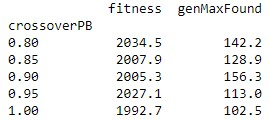
\includegraphics[width=0.3\textwidth]{CXMean}}}
\qquad
\subfloat[Median Fitness]{{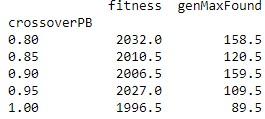
\includegraphics[width=0.3\textwidth]{CXMedian}}}
\caption{Crossover Probability Data}
\label{fig:CXRateFit}
\end{figure}

We find our highest value of 2081 at a 0.8 crossover probability. Applying a Shapiro-Wilk test, we get a value of 0.71 indicating a normal distribution allowing us to take our mean value of 2034. A crossover probability of 0.95 proves very similar mean and median and a very similar Shapiro-Wilk result of 0.71. With both showing a normal distribution, we apply a an independent t test with a result of 0.0 indicating there is no large difference between the sets in terms of fitness. We can see the trend that the higher the crossover probability, the quicker the maximum fitness is found. This is not relevant to the goal of the algorithm so we choose to discount it.
Subsequent experiments use a 0.8 crossover probability.


\subsection{Tournament Size Effect on Fitness}
We test the effect of tournament size on fitness by running the algorithm with a tournament size of 1 to 4 in a step of 1. At each size, the algorithm is run 10 times and the best fitness in each run recorded. Results are shown in Fig \ref{fig:TournamentSizeFit}.
\begin{figure}
\centering
\subfloat[Mean Fitness]{{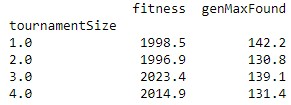
\includegraphics[width=0.3\textwidth]{TSMean}}}
\qquad
\subfloat[Median Fitness]{{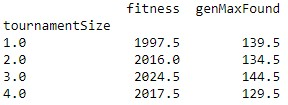
\includegraphics[width=0.3\textwidth]{TSMedian}}}
\caption{Tournament Size Data}
\label{fig:TournamentSizeFit}
\end{figure}

We find our highest fitness value of 2097 with a tournament size of 3. We find a normality of 0.58 for tournament size 3 indicating a normal distribution. The highest mean in the set shows the advantage of this tournament size. Similar results are presented by tournament size 4 which has a normality of 0.48. This is close enough to being a normal distribution that we choose to use an individual t-test to compare sizes. The result is 0.68, indicating some similiarity. We would expect average performances to be fairly similar across these tournament sizes over many runs.
Tournament size 3 delivered our highest fitness value found but tournament size 4 would likely produce similar results, given enough runs.

\subsection{Best Solution Found}
The best solution found, shown in section \ref{appendix:a}, has a value of 2097 with the following settings. POPSIZE=250, MUTPB=0.2, CXPB=0.8, TOURNSIZE=3.

\section{Evaluation}
From the initial problem statement, it is clear that a single best solution would be the goal of the implementation. Subsequently, we needed to take care in analysis as outlier data could promise false improvements and we feel that our experiments and analysis demonstrated that we could back up our decisions. The use of gradual continous experiments on our input parameters allowed us to gradually raise our solution from approximately 1900 to 2097, a marked increase. Unfortunately, there was not room in this report to also experiment with parameters such as number of iterations.

We were also unable to experiment with how our initial seeding mechanism effected the fitness of our solutions. Involving problem-specific knowledge changed the algorithm from being general purpose to being more specialised. We chose to make this change due to the positive effects on fitness we observed in single runs of the algorithm but failing to properly analyse this effect means that we may have hampered the algorithm's performance unknowingly.

We feel that some of our experiments were not thorough enough. Population size, mutation rate and crossover probability showed promising results at the lower/upper bounds of what we tested. More thorough testing should have been done to determine if the true optimal value lay beyond these bounds or on them.

Our initial approach of using an indirect permutation representation worked well. It allowed us to effectively ignore the constraint of team size and simplified the rules needed to build a solution from an individual. However, it should be noted that breaking the constraint of team size is a potential path to diversity that is disallowed in this implementation, potentially causing our solutions to perform poorly and we could not test this without a significant rework.
Our fitness function performed well, in terms of penalty application. All highest fitness solutions tested passed all constraints, meaning that our penalty was never too small and our highest fitness with a maxed out budget of £100 indicates that we did not out right remove invalid solutions from the pool.

We feel that we could have selected a better selection mechanism with more research. We briefly trialed a roulette mechanism to disappointing results and chose to work with something familar whose parameters we understood.

Future improvements could be made to our mutation operator. It currently tries to maintain one constraint while allowing others to be broken. This helps the diversity of our population and future work could investigate the effect of maintaining constraints in mutation. Additionally, the mutation operator could be made to replace low value genes to encourage quicker convergence if a fast solution were needed.

The choice of using an evolutionary algorithm allowed us to tune parameters systematically. However, while we ended with a very high fitness solution, this was an outlier requiring many runs to attain. The mean of the set of runs from which this outlier was obtained was 74 lower than the outlier. Our approach is likely to give high fitness values but cannot reliably give the highest fitness values possible.

\section{Appendix}
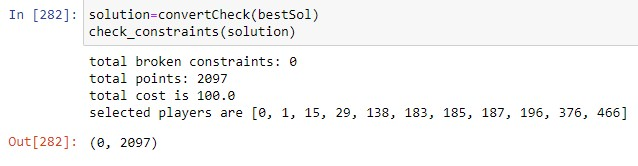
\includegraphics[width=\textwidth]{bestSolution}
\label{appendix:a}
\bibliographystyle{apacite}
\bibliography{bibliography}
\end{document}